\documentclass{beamer}

%%%%%%%%%%%%%%%%%%%%%%%%%%%%%%%%%%%%%%%
%   Language abstraction commands     %
%%%%%%%%%%%%%%%%%%%%%%%%%%%%%%%%%%%%%%%

% spacing
\newcommand{\gap}{\quad\quad}
\newcommand{\biggap}{\quad\quad\quad}
\newcommand{\nextline}{\\ \\}
\newcommand{\htabwidth}{0.5cm}
\newcommand{\tabwidth}{1cm}
\newcommand{\htab}{\hspace{\htabwidth}}
\newcommand{\tab}{\hspace{\tabwidth}}
\newcommand{\linesep}{\ \hrulefill \ \smallskip}

\newcommand{\mi}[1]{\mathit{#1}}

% misc symbols
\newcommand{\dhd}{\!\!\!\!\!\rightarrow}
\newcommand{\Dhd}{\!\!\!\!\!\Rightarrow}
\newcommand{\ts}{\,\vdash\,}
\newcommand{\la}{\langle}
\newcommand{\ra}{\rangle}
\newcommand{\eg}{{\em e.g.}}

% misc identifiers
\newcommand{\dom}{\mbox{\sl dom}}
\newcommand{\fn}{\mbox{\sl fn}}
\newcommand{\bn}{\mbox{\sl bn}}
\newcommand{\sig}{\mbox{\sl sig}}
\newcommand{\IF}{\mbox{\mathem if}}
\newcommand{\OTHERWISE}{\mbox{\mathem otherwise}}
\newcommand{\expand}{\prec}
\newcommand{\weakexpand}{\prec^W}
\newcommand{\spcomma}{~,~}

%% Relations
% Subtype 
\newcommand{\sub}{<:}
% Type assignment
\newcommand{\typ}{:}
% reduction
\newcommand{\reduces}{\;\rightarrow\;}
% well-formedness
\newcommand{\wf}{\;\mbox{\textbf{wf}}}
\newcommand{\nswf}{\mbox{\textbf{wf}}}
\newcommand{\wfe}{\;\mbox{\textbf{wfe}}}
\newcommand{\nswfe}{\mbox{\textbf{wfe}}}

%% Operators
% Type selection
\newcommand{\tsel}{\#}
% Function type
\newcommand{\tfun}{\rightarrow}
\newcommand{\dfun}[3]{(#1\!:\!#2) \Rightarrow #3}
% Conjunction
\newcommand{\tand}{\wedge}
% Disjunction
\newcommand{\tor}{\vee}
% Singleton type suffix
\newcommand{\sing}{.\textbf{type}}

%% Syntax
% Header for typing rules
\newcommand{\judgement}[2]{{\bf #1} \hfill #2}
% Widening
\newcommand{\wid}[2]{#1 : #2}
% Refinement
\newcommand{\refine}[2]{\left\{#1 \Rightarrow #2 \right\}}
\newcommand{\mlrefine}[2]{\{#1 \Rightarrow #2 \}}
% Field definitions
\newcommand{\ldefs}[1]{\left\{#1\right\}}
\newcommand{\mlldefs}[1]{\{#1\}}
% Member sequences
\newcommand{\seq}[1]{\overline{#1}}
% Lambda
\newcommand{\dabs}[3]{(#1\!:\!#2)\Rightarrow #3}
\newcommand{\abs}[3]{\lambda #1\!:\!#2.#3}
% Method Application
\newcommand{\mapp}[3]{#1.#2(#3)}
% Substitution
\newcommand{\subst}[3]{[#1/#2]#3}
% Object creation
\newcommand{\new}[3]{\textbf{val }#1 = \textbf{new }#2 ;\; #3}
\newcommand{\mlnew}[3]{\textbf{val }#1 = \textbf{new }#2 ;\;\\&#3}
%\renewcommand{\new}[3]{#1 \leftarrow #2 \,\textbf{in}\, #3}
% Field declaration
\newcommand{\Ldecl}[3]{#1 : #2..#3}%{#1 \operatorname{>:} #2 \operatorname{<:} #3}
\newcommand{\ldecl}[2]{#1 : #2}
\newcommand{\mdecl}[3]{#1 : #2 \tfun #3}
% Top and Bottom
\newcommand{\Top}{\top}%{\textbf{Top}}
\newcommand{\Bot}{\bot}%\textbf{Bot}}
% Environment extension
%\newcommand{\envplus}[1]{\uplus \{ #1 \}}
\newcommand{\envplus}[1]{, #1}
% Reduction
\newcommand{\reduction}[4]{#1 \operatorname{|} #2 \reduces #3 \operatorname{|} #4}

% Sugar
\newcommand{\arrow}[2]{#1\rightarrow_s#2}
\newcommand{\fun}[4]{\textbf{fun } (#1:#2)\;#3\;#4}
\newcommand{\app}[2]{(\textbf{app }#1\;#2)}
\newcommand{\mlapp}[2]{(\textbf{app }#1\;\\&#2)}
\newcommand{\cast}[2]{(\textbf{cast }#1\;#2)}

\newcommand{\lindent}{\hspace{-4mm}}

% Logical relations
\newcommand{\relv}[4]{\mathcal{V}_{#1;#2;#3}\llbracket#4\rrbracket}
\newcommand{\rele}[4]{\mathcal{E}_{#1;#2;#3}\llbracket#4\rrbracket}
\newcommand{\rels}[3]{\mathcal{\supseteq}_{#1}\llbracket#2;#3\rrbracket}
\newcommand{\relg}[3]{\mathcal{\supseteq^!}_{#1;#2}\llbracket#3\rrbracket}
\newcommand{\irred}[2]{\text{irred }(#1,#2)}
\newcommand{\andl}{\;\wedge\;}
\newcommand{\orl}{\vee}
\newcommand{\impliesl}{\rightarrow}
\newcommand{\reductionl}[5]{#1 \operatorname{|} #2 \;\rightarrow^{#5}\; #3 \operatorname{|} #4}
\newcommand{\ds}{\,\vDash\,}

\usepackage{bcprules}

\usepackage{minted}
\usemintedstyle{eclipse}
% I added & and | as Scala keywords in Pygments:
%% diff -r 121c75491e0d pygments/lexers/jvm.py
%% --- a/pygments/lexers/jvm.py	Tue May 06 20:21:16 2014 -0700
%% +++ b/pygments/lexers/jvm.py	Sat May 10 19:21:51 2014 +0200
%% @@ -259,7 +259,7 @@
%%               u'lazy|match|new|override|pr(?:ivate|otected)'
%%               u'|re(?:quires|turn)|s(?:ealed|uper)|'
%%               u't(?:h(?:is|row)|ry)|va[lr]|w(?:hile|ith)|yield)\\b|'
%% -             u'(<[%:-]|=>|>:|[#=@_\u21D2\u2190])(\\b|(?=\\s)|$)', Keyword),
%% +             u'(<[%:-]|\\&|(\\|)|=>|>:|[#=@_\u21D2\u2190])(\\b|(?=\\s)|$)', Keyword),
%%              (u':(?!%s)' % op, Keyword, 'type'),
%%              (u'%s%s\\b' % (upper, idrest), Name.Class),
%%              (r'(true|false|null)\b', Keyword.Constant),


\usepackage{verbatim}
\usepackage{hyperref}

\useoutertheme{infolines}
\setbeamertemplate{headline}{}
\setbeamertemplate{footline}{
  \hfill
  \usebeamercolor[fg]{page number in head/foot}
  \usebeamerfont{page number in head/foot}
  \insertpagenumber\kern1em\vskip10pt
}
\setbeamertemplate{navigation symbols}{}

\title{The {\bf DOT} Calculus}
\subtitle{({\bf D}ependent {\bf O}bject {\bf T}ypes)}
\author{Nada Amin}
\institute{Scala Days}
\date{June 18, 2014}

\AtBeginSection{
  \begin{frame}
    \begin{center}
      \structure{\Huge \insertsection}
    \end{center}
  \end{frame}
}

\begin{document}

\frame{\titlepage}

\begin{frame}[fragile]{DOT: Dependent Object Types}
\begin{itemize}
\item DOT is a core calculus for path-dependent types.
\item Goals
\begin{itemize}
\item simplify Scala's type system by desugaring to DOT
\item simplify Scala's type inference by relying on DOT
\item prove that DOT is type-safe
\end{itemize}
\end{itemize}
\end{frame}

\begin{comment} (abstract)
The DOT (Dependent Object Types) calculus attempts to ground Scala's
type system in fewer, but powerful, constructs. In this talk I will
describe what these constructs are, and how they relate to Scala's
current type system. I will also show how DOT simplifies type
inference. Finally, I will touch upon the challenges in the
meta-theory.
\end{comment}

\section{Types in Scala and DOT}

\begin{frame}[fragile]{Types in Scala}
\begin{description}[functional]
\item[modular]\begin{description}[higher-kinded types]
\item[named type]\mint{scala}|scala.collection.BitSet|
\item[compound type]\mint{scala}|Channel with Logged|
\item[refined type]\mint{scala}|Channel { def close(): Unit } |
\end{description}
\item[functional]\begin{description}[higher-kinded types]
\item[parameterized type]\mint{scala}|List[String]|
\item[existential type]\mint{scala}|List[T] forSome { type T }|
\item[higher-kinded type]\mint{scala}|List|
\end{description}
\end{description}
\begin{comment}
too many orthogonal concepts?
can we simplify by keeping only the modular features?
\end{comment}
\end{frame}

\begin{frame}[fragile]{Reducing Functional to Modular?}
\begin{itemize}
\item type parameter to type member\\
\mint{scala}|class List[Elem] {} /*vs*/ class List { type Elem }|
\item parameterized type to refined type\\
\mint{scala}|List[String] /*vs*/ List { type Elem = String }|
\item existential type?\\
\mint{scala}|List[_] /*or*/ List[T] forSome { type T } /*~vs~*/ List|
\item higher-kinded type?\\
\mint{scala}|List /*~vs~*/ List|
\end{itemize}
\end{frame}

\begin{frame}[fragile]{Bonus: {\bf D}on't {\bf R}epeat {\bf Y}ourself}
\begin{minted}{scala}
         new HashMap[String, List[Int]]
with SynchronizedMap[String, List[Int]]

           /*vs*/

         new HashMap[String, List[Int]]
with SynchronizedMap
\end{minted}
\end{frame}

\begin{frame}[fragile]{Type Members and Modularity (Example)}
\begin{minted}{scala}
trait Symbols {
  type Type
  // a symbol has a type ...
  trait Symbol { def tpe: Type }
}
trait Types {
  type Symbol
  // ... and a type has a symbol
  trait Type { def sym: Symbol }
}
// ... but the references are not hard-coded!
// putting the cake together:
trait SymbolTable extends Symbols with Types
\end{minted}
\end{frame}

\begin{frame}[fragile]{Type Members and Data Abstraction (Example)}
\begin{minted}{scala}
trait HeapModule {
  type Heap
  type Elem
  def ord: Ordering[Elem]
  def empty: Heap
  def isEmpty(h: Heap): Boolean
  def insert(x: Elem, h: Heap): Heap
  def findMin(h: Heap): Elem
  def deleteMin(h: Heap): Heap
  def merge(h1: Heap, h2: Heap): Heap
}
trait BinomialHeapModule extends HeapModule {
  type Rank = Int
  case class Node(x: Elem, r: Rank, c: List[Node])
  override type Heap = List[Node]
  // ... implementation ...
}
\end{minted}
\end{frame}

\begin{frame}[fragile]{Path-Dependent Types and Binary Methods (Example)}
\begin{minted}{scala}
val m1: HeapModule = ...
val m2: HeapModule = ...
// in Scala REPL
> m1.merge(m1.empty, m2.empty)
// error: type mismatch;
// found   : m2.Heap
// required: m1.Heap
//              m1.merge(m1.empty, m2.empty)
//                                    ^
\end{minted}
\end{frame}

\begin{frame}[fragile]{Types in DOT}
\begin{description}[declarations]
\item[types]\mint{scala}|S, T, U|
\begin{description}[path-dependent type]
\item[path-dependent type]\mint{scala}|p.L|
\item[refined type]\mint{scala}|T { z => D }|
\item[intersection]\mint{scala}|T & T|
\item[union]
\begin{minted}{scala}
T | T
\end{minted}
\item[top]\mint{scala}|Any|
\item[bottom]\mint{scala}|Nothing|
\end{description}
\item[declarations]\mint{scala}|D|
\begin{description}[path-dependent type]
\item[type declaration]\mint{scala}|type L >: S <: U|
\item[field declaration]\mint{scala}|val l: U|
\item[method declaration]\mint{scala}|def m(x: S): U|
\end{description}
\end{description}
\end{frame}

\section{Type Inference}

\begin{frame}[fragile]{Type Inference in Scala (Least Upper Bound?)}
\begin{minted}{scala}
trait A { type T <: A }
trait B { type T <: B }
trait C extends A with B { type T <: C }
trait D extends A with B { type T <: D }
// in Scala, lub(C, D) is an infinite sequence
A with B { type T <: A with B { type T <: ... } }

// in Scala REPL
> val o = if (true) (new C{}) else (new D{})
o: A with B{type T <: A with B} = ...
> val o:A with B{type T<:A with B {type T<:A with B}} =
          if (true) (new C{}) else (new D{})
o: A with B{type T <: A with B{type T <: A with B}} = ...
\end{minted}
\end{frame}

\begin{frame}[fragile]{Type Inference in Scala (Working too Hard too Soon?)}
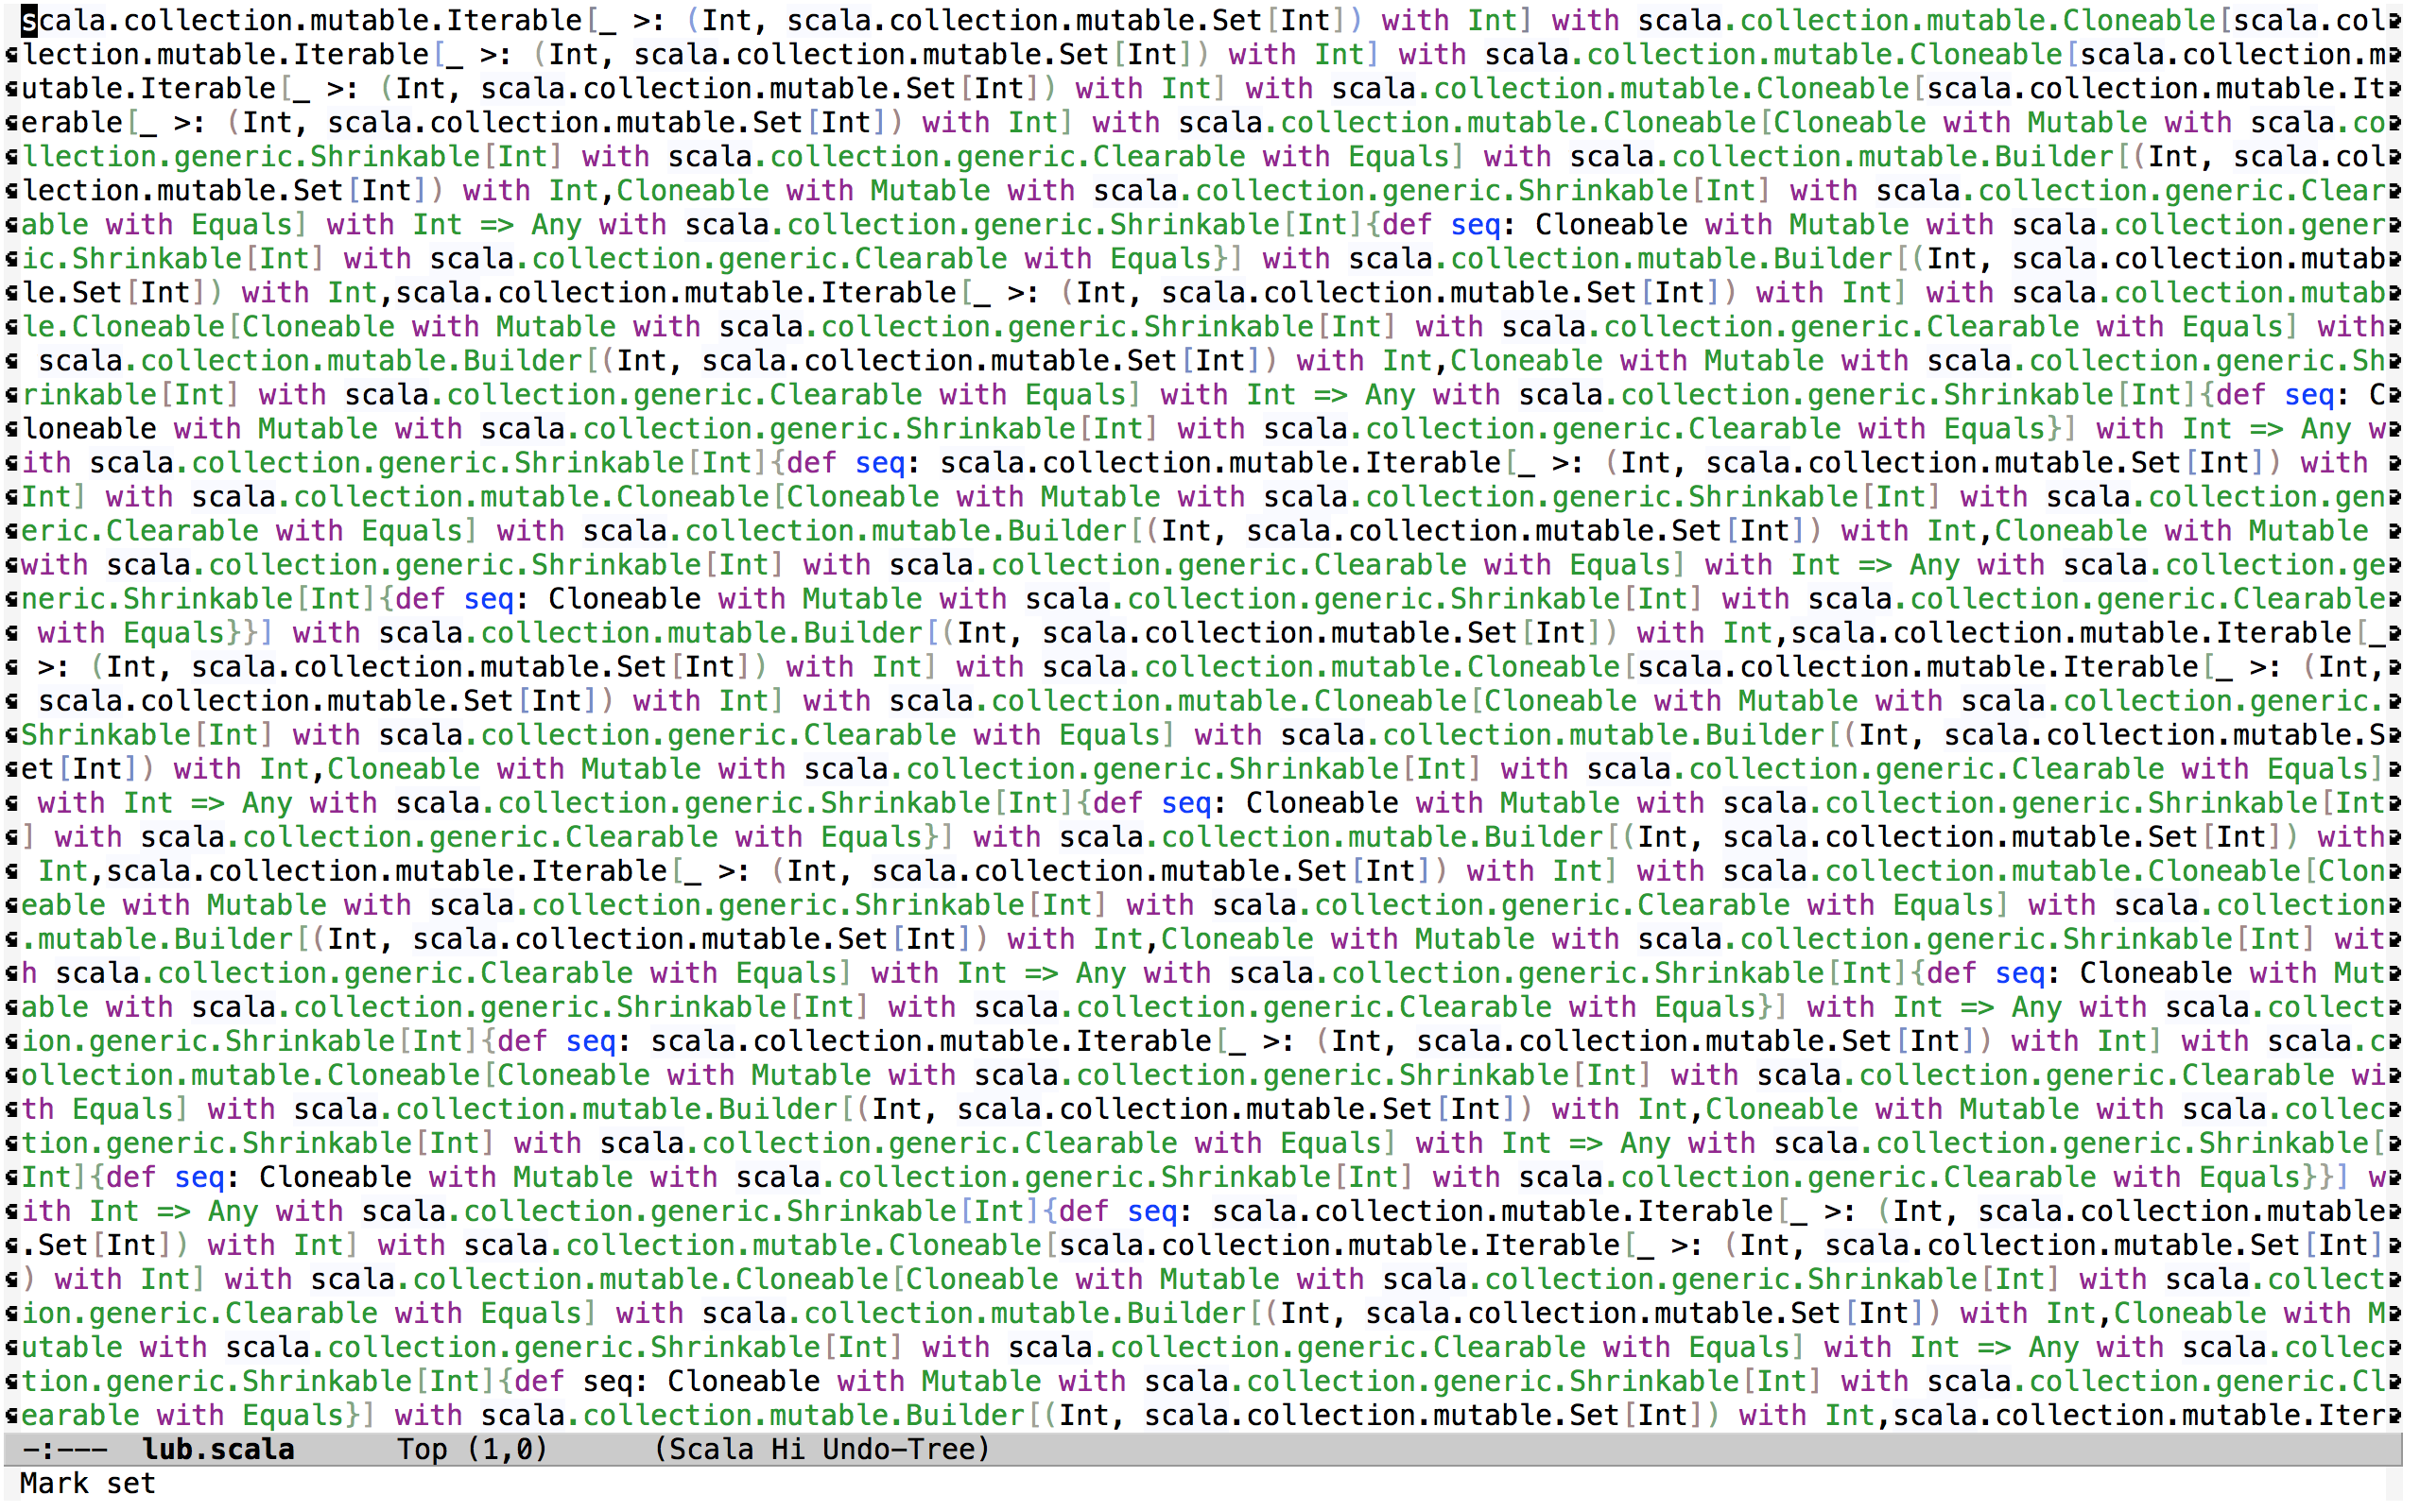
\includegraphics[width=\textwidth]{lub1.png}
\end{frame}

\begin{frame}[fragile]{Type Inference in Scala (Working too Hard too Soon?)}
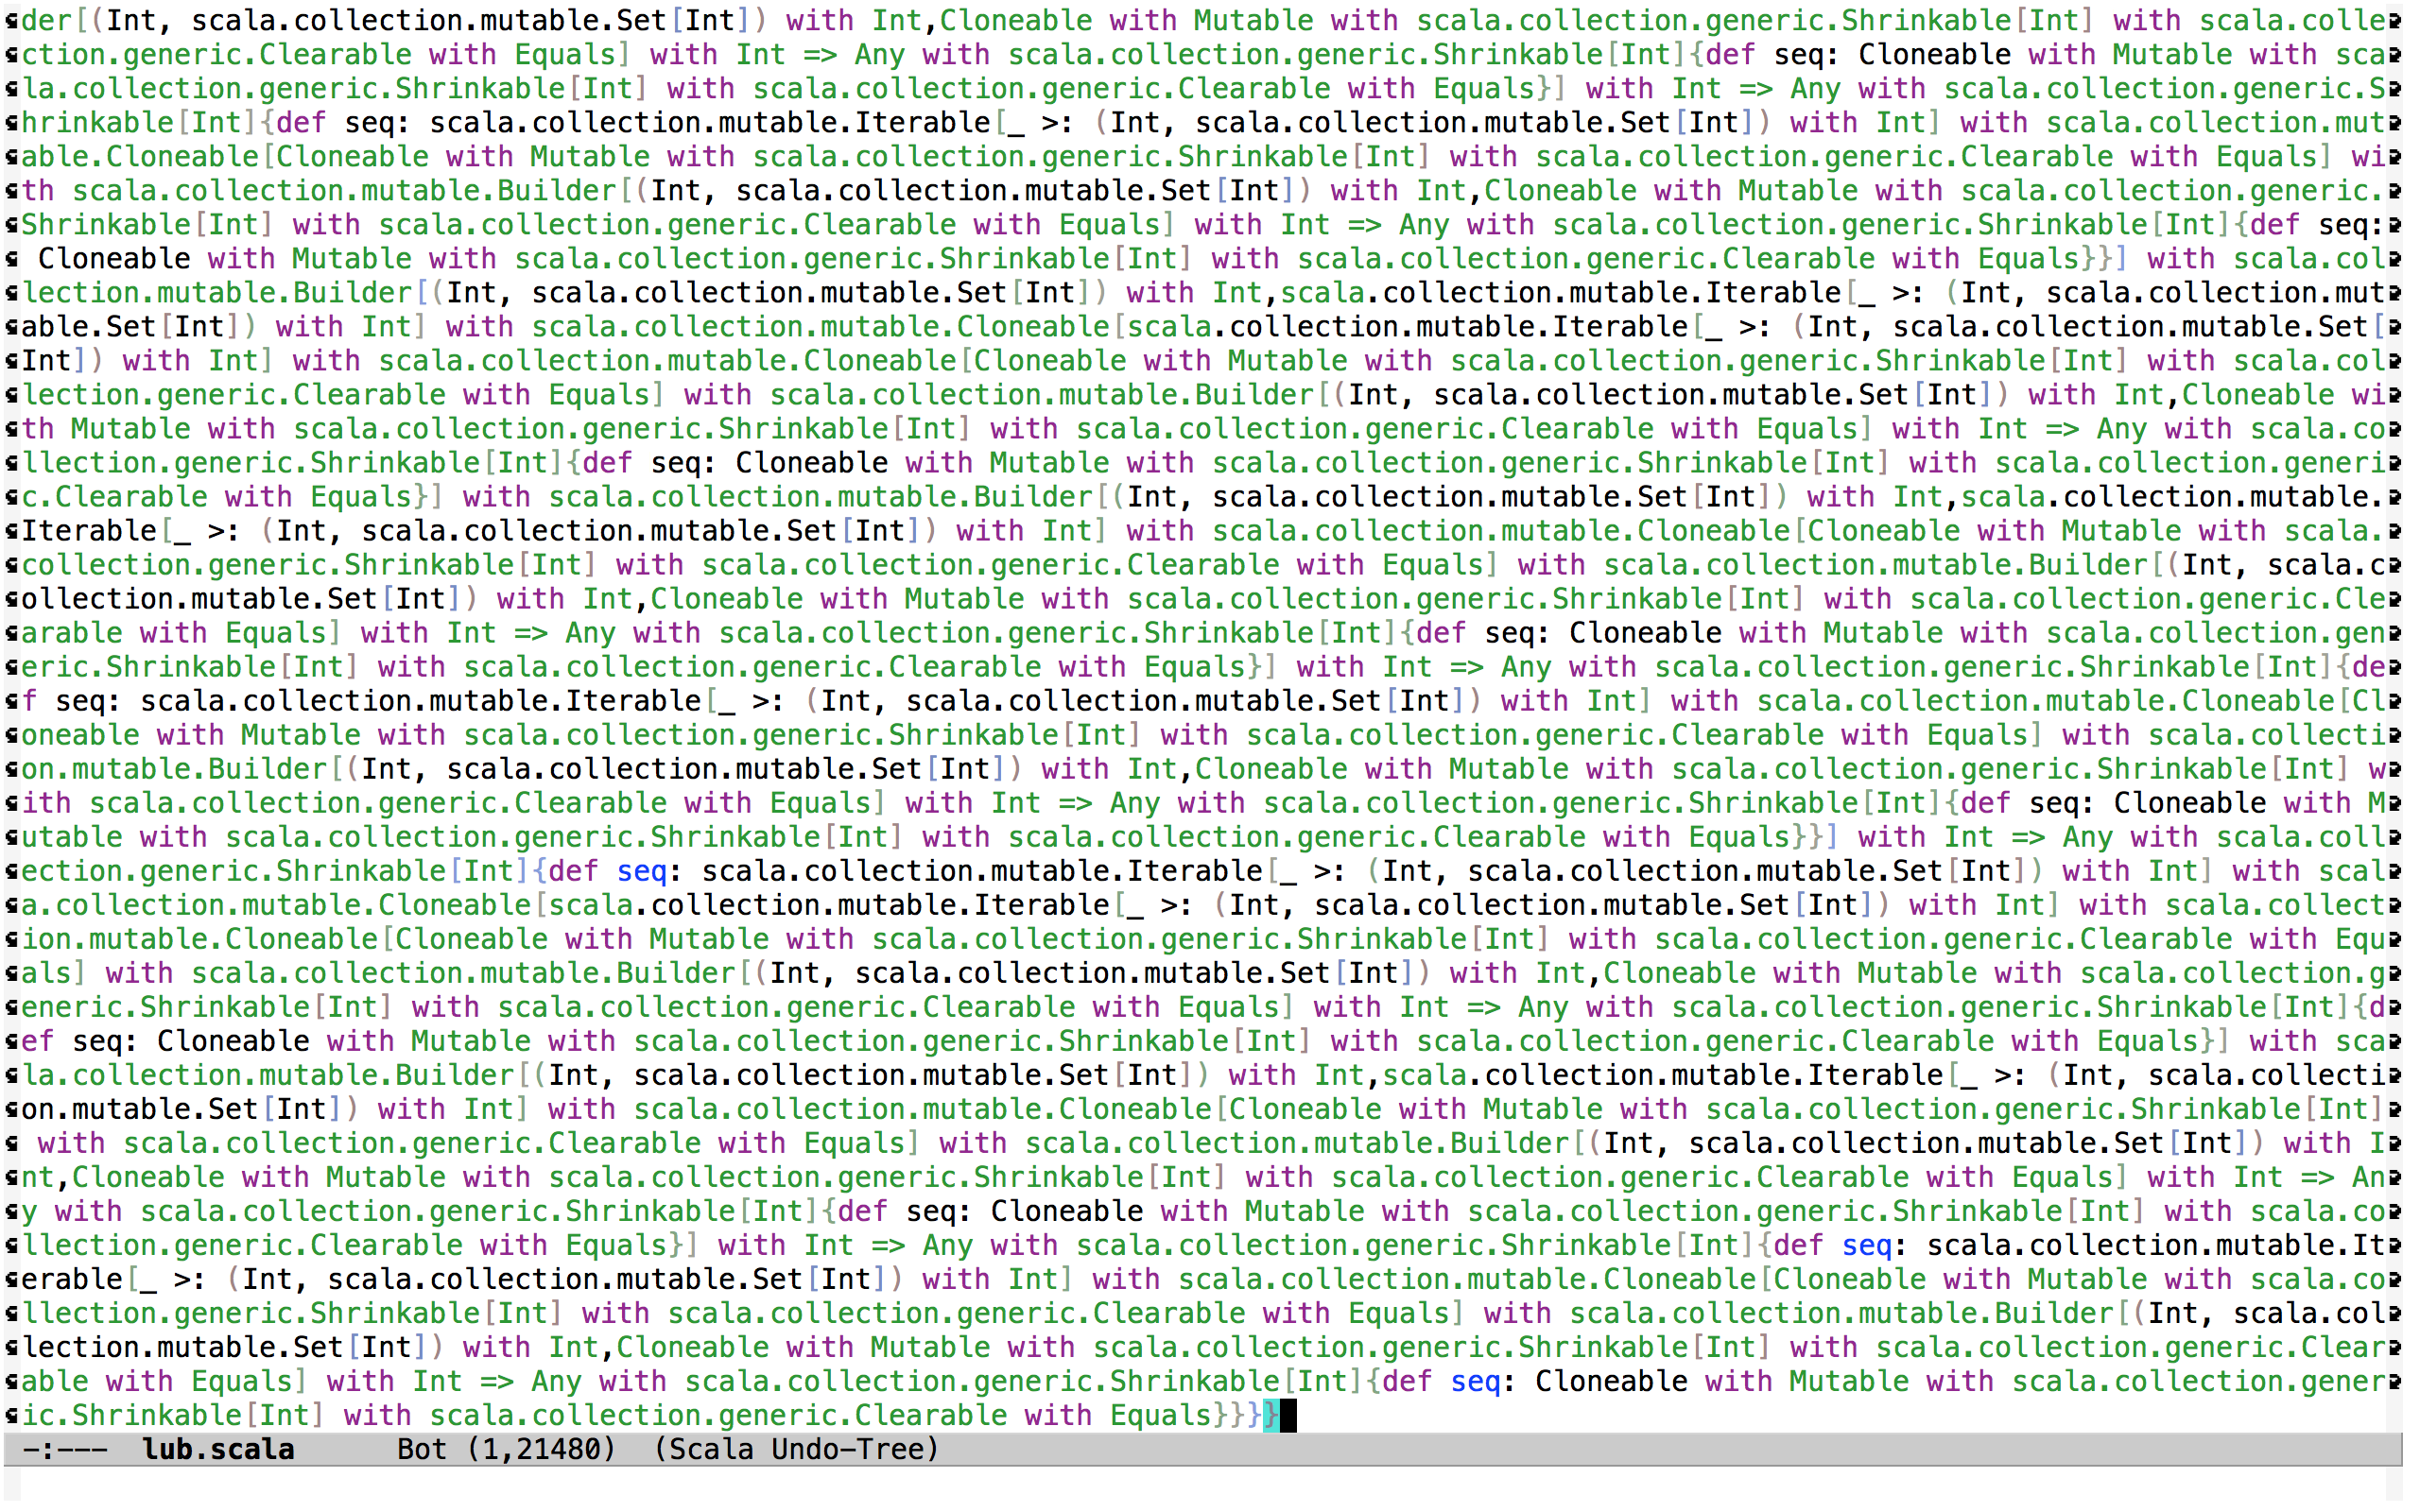
\includegraphics[width=\textwidth]{lub2.png}
\end{frame}

\begin{frame}[fragile]{Type Inference in Scala (Working too Hard too Soon?)}
\begin{minted}{scala}
import scala.collection.mutable.{Map => MMap, Set => MSet}
val ms: MMap[Int, MSet[Int]] = MMap.empty

// in Scala REPL
> if (!ms.contains(1)) ms += 1 -> MSet(1) else ms(1) += 1
res0: ... (796 characters) ...
> :t res0
    : ... (21481 characters) ...
\end{minted}
\begin{itemize}
\item Inspired by a bug report\\
\href{https://issues.scala-lang.org/browse/SI-5862}{SI-5862}: very slow compilation due to humonguous LUB.
\item The character lengths reported are for Scala 2.11 ({\em after} the fix).
\item In Dotty, type inference can be lazy thanks to the native unions (for least upper bounds) and intersections (for greatest lower bounds) of the core calculus (DOT).
\end{itemize}
\end{frame}

\section{Meta-Theory}

\begin{frame}[fragile]{Type Safety: ``Well-typed programs can't go wrong.''}
\begin{minted}{javascript}
// ... at least in some ways ...
// JavaScript REPL
> var x = {foo: 'hello'}
undefined
> x.foo
"hello"
> x.bar
undefined
> x.bar.boo
// TypeError: Cannot read property 'boo' of undefined
> x.foo('hello')
// TypeError: string is not a function
\end{minted}
\end{frame}

\begin{frame}[fragile]{Type Safety: Syntactic Recipe (Concepts)}
\begin{description}[preservation]
\item[small-step] operational semantics (``show all your steps'')
\item[irreducible] terms, stuck terms vs values
\item[progress] theorem: if a term type-checks, then it can take a step or it is a value (but not stuck!)
\item[preservation] theorem: if a term type-checks and steps, then the new term also type-checks with the same type (or subtype)
\item[type safety] = progress + preservation
\end{description}
\end{frame}

\begin{frame}[fragile]{Preservation Challenge: Branding}
\begin{minted}{scala}
trait Brand {
  type Name
  def id(x: Any): Name
}
// in REPL
val brand: Brand = new Brand {
  type Name = Any
  def id(x: Any): Name = x
}
brand.id("hi"): brand.Name // ok
"hi": brand.Name // error but probably sound
val brandi: Brand = new Brand {
  type Name = Int
  def id(x: Any): Name = 0
}
brandi.id("hi"): brandi.Name // ok
"hi": brandi.Name // error and probably unsound
\end{minted}
\end{frame}

\begin{frame}[fragile]{Theory: Subtyping of Path-Dependent Types}
\begin{itemize}
\item \mint{scala}|/*If*/ p.L /*has lower bound*/ Sp /*and upper bound*/ Up|
\begin{itemize}
\item \mint{scala}|S   <: p.L /*if*/ S   <: Sp|
\item \mint{scala}|p.L <: U   /*if*/ Up  <: U|
\end{itemize}
\end{itemize}
\end{frame}

\begin{frame}[fragile]{Preservation Challenge: Path equality}
\begin{minted}{scala}
trait B { type X; val l: X }
val b1: B = new B { type X = String; val l: X = "hi" }
val b2: B = new B { type X = Int;    val l: X = 0    }
trait A { val i: B }
val a = new A { val i: B = b1 }
println(a.i.l : a.i.X) // ok
println(b1.l  : b1.X)  // ok
println(b1.l  : a.i.X) // error: type mismatch;
// found   : b1.l.type (with underlying type b1.X)
// required: a.i.X
// abstractly, would need to show
Any  <: Nothing // lattice collapse!
// to show
b1.X <: a.i.X
// because
U of b1.X = Any <: Nothing = S of a.i.X
println(b2.l  : a.i.X) // error and probably unsound
\end{minted}
\end{frame}

\begin{frame}[fragile]{Challenge: Subtyping Transitivity}
\begin{itemize}
\item \mint{scala}|S <: T <: U /*imply*/ S <: U|
\end{itemize}
\end{frame}

\begin{frame}[fragile]{Subtyping Transitivity and Path-Dependent Types}
\begin{itemize}
\item \mint{scala}|S <: p.L <: U|
\item \mint{scala}|p.L /*has lower bound*/ Sp /*and upper bound*/ Up|
\item \mint{scala}|S  <: Sp|
\item \mint{scala}|Up <: U|
\end{itemize}
\end{frame}

\begin{frame}[fragile]{Subtyping Transitivity and Path-Dependent Types with Bad Bounds}
\begin{itemize}
\item \mint{scala}|/*Suppose*/ p.L /*has bad bounds, e.g.*/|
\begin{itemize}
\item \mint{scala}|p.L /*has lower bound*/ Any /*and upper bound*/ Nothing|
\item \mint{scala}|S  <: Any     /*for any*/ S|
\item \mint{scala}|U  <: Nothing /*for any*/ U|
\item \mint{scala}|S <: p.L <: U /*imply*/ S <: U /*for any*/ S, U|
\end{itemize}
\item Lattice collapse!
\end{itemize}
\end{frame}

\begin{frame}[fragile]{Path-Dependent Types (Recap Example)}
\begin{minted}{scala}
trait Animal { type Food; def gets: Food
               def eats(food: Food) {}; }
trait Grass; trait Meat
trait Cow extends Animal with Meat {
  type Food = Grass; def gets = new Grass {} }
trait Lion extends Animal {
  type Food = Meat;  def gets = new Meat {} }
val leo = new Lion {}
val milka = new Cow {}
leo.eats(milka) // ok
val lambda: Animal = milka
lambda.eats(milka) // type mismatch
// found : Cow
// required: lambda.Food
lambda.eats(lambda.gets) // ok
\end{minted}
\end{frame}

\begin{frame}[fragile]{Path-Dependent Types (Recap Example Continued)}
\begin{minted}{scala}
def share(a1: Animal)(a2: Animal)
         (bite: a1.Food with a2.Food) {
  a1.eats(bite)
  a2.eats(bite)
}
val simba = new Lion {}
share(leo)(simba)(leo.gets) // ok
share(leo)(lambda)(leo.gets) // error: type mismatch
// found : Meat
// required: leo.Food with lambda.Food

// Observation:
// We don't know whether the parameter type of
share(lambda1)(lambda2)_
// is realizable until run-time.
\end{minted}
\end{frame}

\begin{frame}[fragile]{Realizability of Intersection Types at Run-Time}
\begin{minted}{scala}
val lambda1: Animal = new Lion {}
val lambda2: Animal = new Cow  {}
lazy val p: lambda1.Food & lambda2.Food = ???
// for illustration, say we re-defined the following:
trait Food { type T }
trait Meat extends Food  { type T = Nothing }
trait Grass extends Food { type T = Any }
// statically
p.T /*has fully abstract bounds*/
// at runtime
lambda1.Food /*is*/ Meat /*&*/ lambda2.Food /*is*/ Grass
p /*has type*/ Meat & Grass
// lower bound is union of lower bounds
p.T /*has lower bound*/ Nothing | Any /*is*/ Any
// upper bound is intersection of upper bounds
p.T /*has upper bound*/ Nothing & Any /*is*/ Nothing
p.T /*has bad bounds at run-time!*/
\end{minted}
\end{frame}

\begin{frame}[fragile]{Summary}
\begin{itemize}
\item DOT is a core calculus for path-dependent types.
\item Benefits for Scala
\begin{itemize}
\item simpler type system
\item better type inference
\item (hopefully) easier reasoning
\end{itemize}
\item Challenges in Meta-Theory
\begin{itemize}
\item type preservation
\begin{itemize}
\item run-time path equality
\item inlining branding
\end{itemize}
\item path-dependent types with ``bad bounds''
\begin{itemize}
\item subtyping transitivity
\item run-time ``bad bounds'' via intersection types
\end{itemize}
\end{itemize}
\end{itemize}
\end{frame}

\section{Thank You!}

\end{document}
